\documentclass[12pt,english]{article}
\usepackage[english]{babel}
\usepackage{graphicx}
\usepackage{amsmath}
\usepackage{adjustbox}
\usepackage{multirow}
\usepackage{subcaption}
\usepackage{amssymb}
\usepackage[hidelinks]{hyperref}
\usepackage{caption}
\usepackage{amsthm}
\usepackage{multicol}
\usepackage{minted}
\usepackage{float}
\usepackage{titling}
\usepackage{soul}
\usepackage{listings}
\usepackage{array}
\graphicspath{ {../img/}}
\selectlanguage{english}
\usepackage[nottoc]{tocbibind}
\usepackage[utf8]{inputenc}
\usepackage{graphicx}
\usepackage[a4paper,left=2cm,right=2cm,top=2.5cm,bottom=2.5cm]{geometry}
\RecustomVerbatimEnvironment{Verbatim}{BVerbatim}{}


\title{Cloud Computing}
\setlength{\droptitle}{10em}
\author{Carlos Sánchez Páez}

\makeindex
\begin{document}


\begin{titlepage}

 \newlength{\centeroffset}
 \setlength{\centeroffset}{-0.5\oddsidemargin}
 \addtolength{\centeroffset}{0.5\evensidemargin}
 \thispagestyle{empty}

 \noindent\hspace*{\centeroffset}
 \begin{minipage}{\textwidth}

  \centering
  
\includegraphics[width=0.75\textwidth]{bme_logo.jpg}\\[1.4cm]

  \textsc{ \Large Cloud Computing\\[3cm]}

  \textsc{\Huge Working with Google Cloud}\\[2cm]

  \begin{figure}[H]
    \centering
    
\includegraphics[width=0.5\textwidth]{../img/logo}
  \end{figure}
 \end{minipage}


 \vspace{3cm}
 \noindent\hspace*{\centeroffset}
 \begin{minipage}{\textwidth}
  \centering

  \textbf{Author}\\ {Carlos Sánchez Páez}\\
  \texttt{http://www.github.com/csp98}\\[0.5cm]
  \textsc{Budapest University of Technology and Economics}\\
  \vspace{1cm}
  \textsc{Academic year 2018-2019}
 \end{minipage}
\end{titlepage}
\thispagestyle{empty}
\newpage
\tableofcontents{}
\thispagestyle{empty}
\newpage

\section{What is Google Cloud Platform?}

Google Cloud Platform (GCP) is a set of Google computing resources. These resources are internally used by the company to develop their own products, such as YouTube, Search, Translate, etc. These services are available to the public via services (public cloud offer).\\

Google Cloud Platform is the third company in the public cloud market (bewind Amazon Web Services and Microsoft Azure). It offers IaaS, SaaS, PaaS, etc. in more than 50 products.\\

\subsection{Main advantages of the platform}

\begin{itemize}
 \item Free customization of the resources of the VM or the possibility of using a template depending on the load that it will have.
 \item Interactive tutorials in the platform to avoid people getting lost.
 \item Project Control Panel to manage the project and study stadistics, metrics, error reporting, etc.
 \item Android \& IOS application to access the control panel from everywhere.
 \item Online terminal in the website or downloadable SDK to work from the system's command-line interface.
 \item Free trial of one year and 300 USD to spend in any product.
\end{itemize}

\begin{figure}[H]
  \centering
  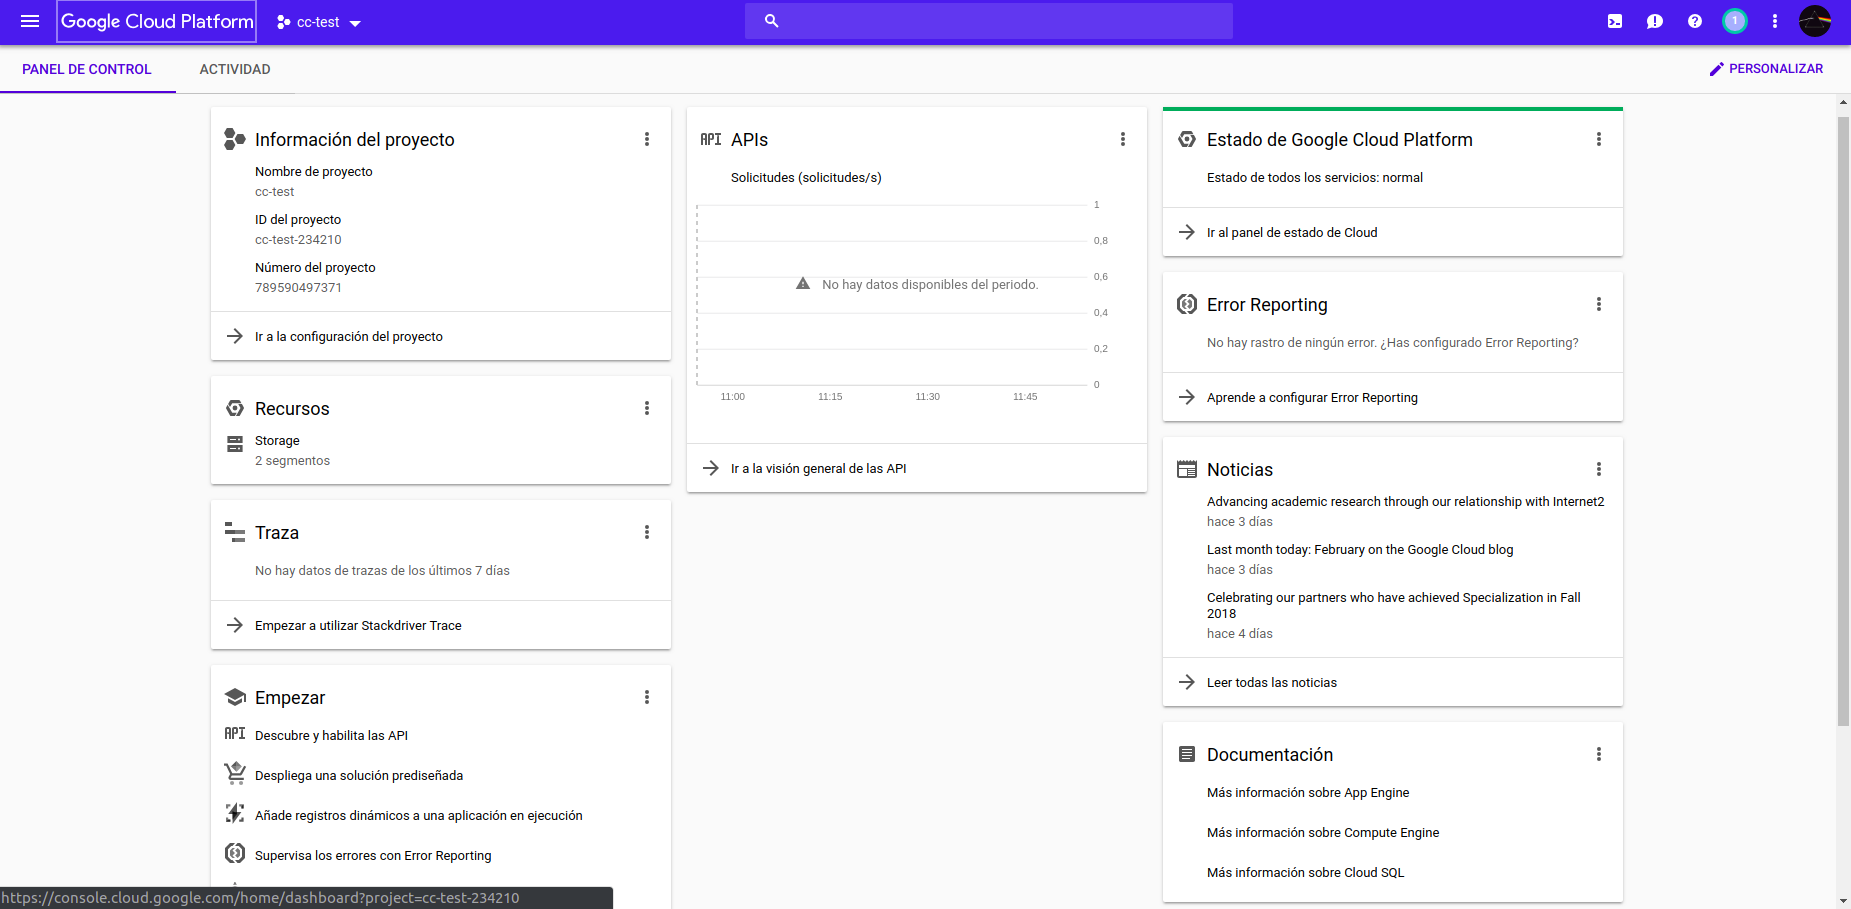
\includegraphics[scale = 0.35]{../img/tutorial/2controlpanel}
  \caption{Project Control Panel}
\end{figure}

\begin{figure}[H]
  \centering
  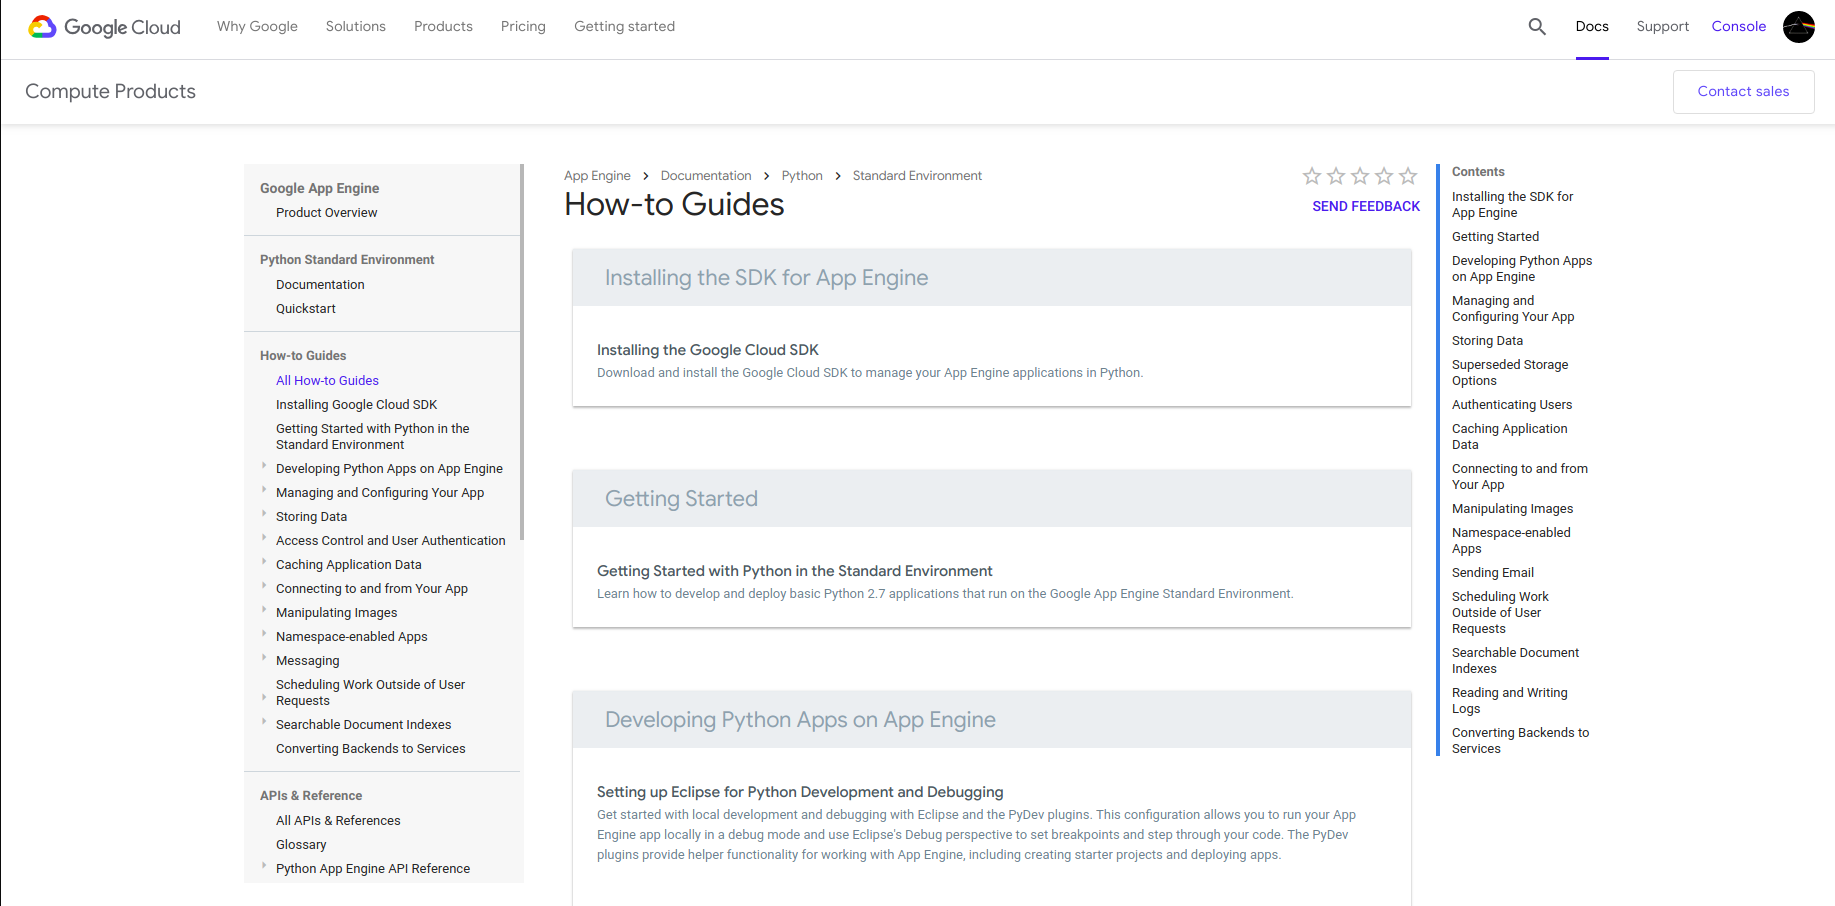
\includegraphics[scale = 0.35]{tutorials.png}
  \caption{Tutorials in the platform}
\end{figure}

\begin{figure}[H]
  \centering
  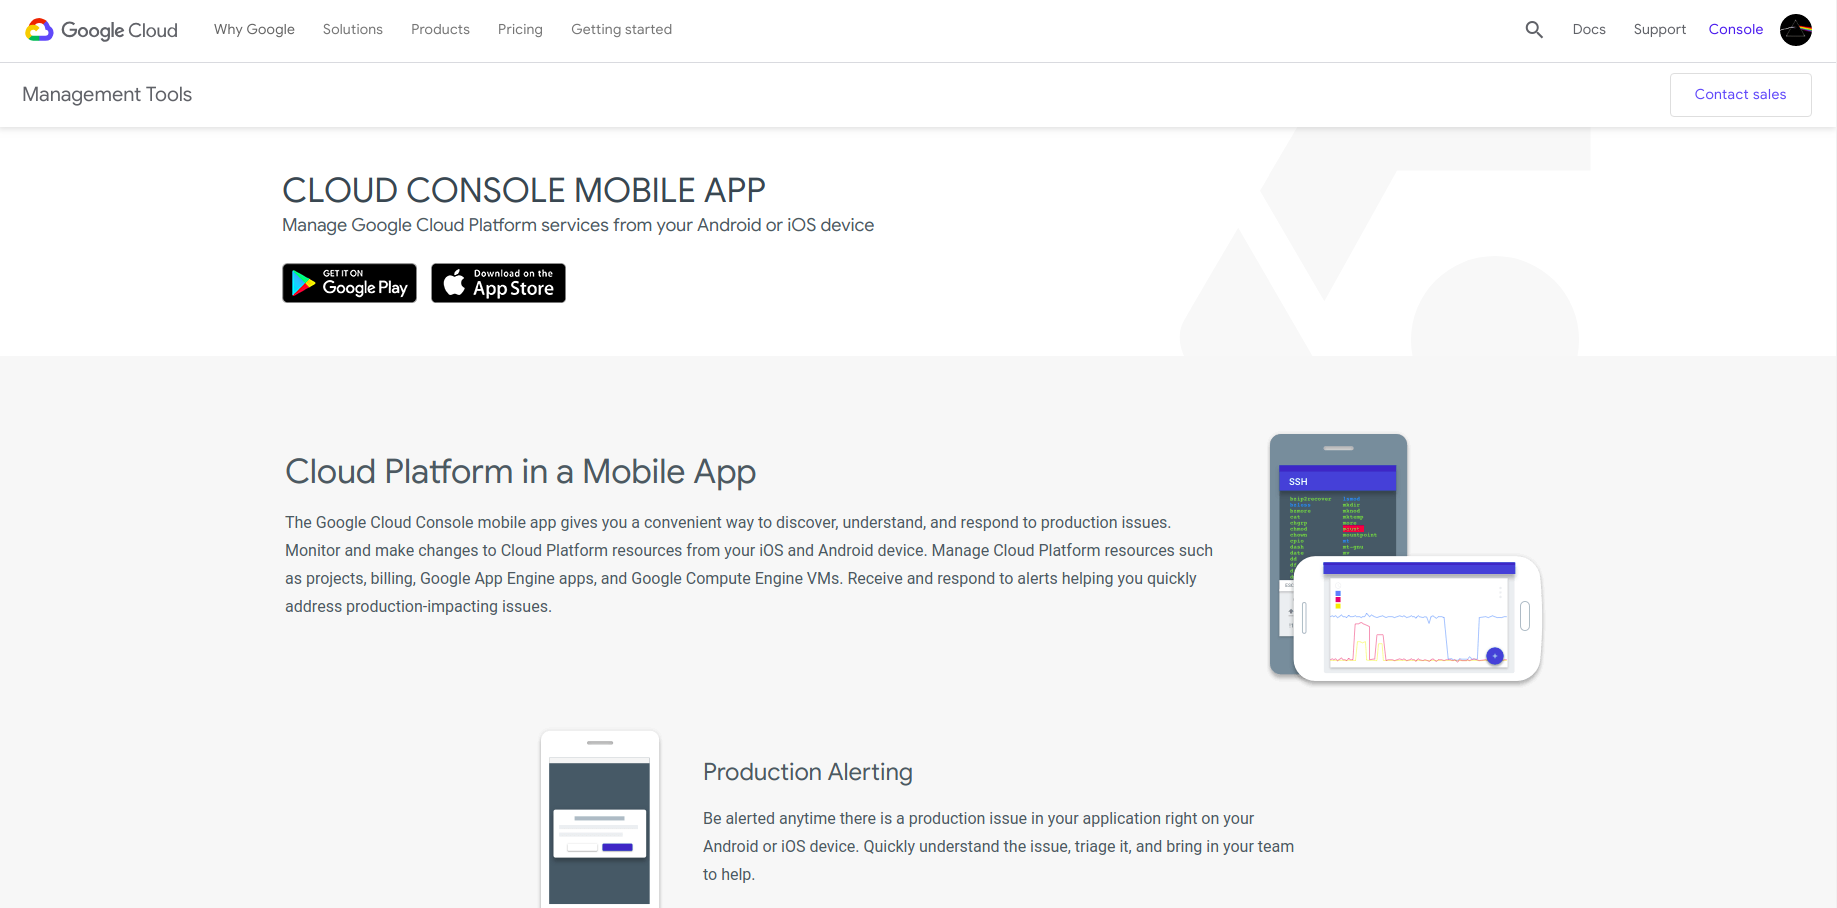
\includegraphics[scale = 0.35]{app.png}
  \caption{Mobile app}
\end{figure}

\newpage

\section{Companies that use it}

A huge amount of companies use GCP. In February 2018, Google reported that it had more than four million paying customers. Some of the most important businesses are:
\begin{itemize}
 \item New York Times.
 \item Twitter.
 \item Ebay.
 \item Telenor.
 \item Paypal.
\end{itemize}

\begin{figure}[H]
  \centering
  
\includegraphics[scale = 0.5]{../img/logos}
  \caption{Companies that use GCP}
\end{figure}

\section{Google Cloud Platform products}

\subsection{Computing}

\begin{itemize}
 \item App Engine: offers scalable apps via Platform as a Service.
 \item Compute Engine allows us to connect to a provisioned machine via SSH (Infrastructure as a Service).
 \item Kubernetes makes possible to run containers, for example Docker ones. Containers pack applications and their dependences and libraries, so that they can be runt in every platform. This is a case of virtualisation where the hypervisor is Docker.
\end{itemize}

\subsection{Networking}

\begin{itemize}
  \item Cloud Armor is used to prevent Denial of Service attacks.
  \item Network Service Tiers optimizes our product by taking the best tier according of what we want to improve: performance or cost.
  \item Load balancing allows applications to automatically scale depending on the demand that they receive.
\end{itemize}

\subsection{Big Data}

\begin{itemize}
  \item Dataprep offers data cleaning and preprocessing.
  \item Dataflow processes the batches.
  \item Genomics is used in bioinformatics.
\end{itemize}

\subsection{Machine Learning}

\begin{itemize}
  \item Vision API recognises objects in an image. It is used in Google Lens.
  \item Speech API is used to transform voice into text. Used in Google Assistant.
  \item Natural Language API extracts information about something mentioned in a text (sentiment, importance in the test, etc.).
  \item Translate API is used in Google Translate.
\end{itemize}

\section{Example of use}

Let's develop and deploy a simple application using App Engine (PaaS). Our source code is very simple, it just shows the sentence "Hello World" in the homepage. Here we can see it:

\begin{figure}[H]
  \centering
  \begin{minted}{python}
  import webapp2
  class MainPage(webapp2.RequestHandler):
  def get(self):
      self.response.headers
      ['Content-Type'] = 'text/plain'
      self.response.write('Hello world!')

  app = webapp2.WSGIApplication([
  ('/', MainPage),
  ], debug=True)


  \end{minted}
  \caption{Source code of the app}
\end{figure}

The first step is creating the project. When doing that, we will be able to select the region for the deployment so that the nearest users have the lowest latency.\\

\begin{figure}[H]
  \centering
  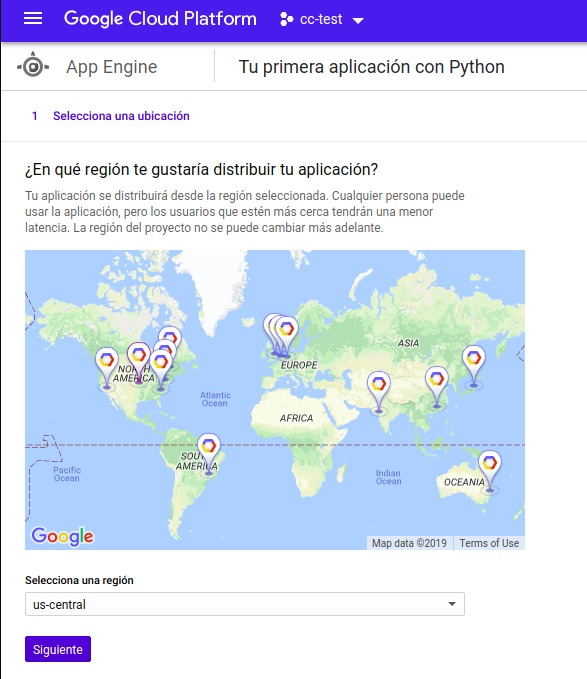
\includegraphics[scale = 0.5]{../img/tutorial/1select_region}
  \caption{Selection of the deployment region}
\end{figure}

 Then, we must set the project up with the command \emph{gcloud config set project <ID>} where ID is the identificator of the project.

 \begin{figure}[H]
   \centering
   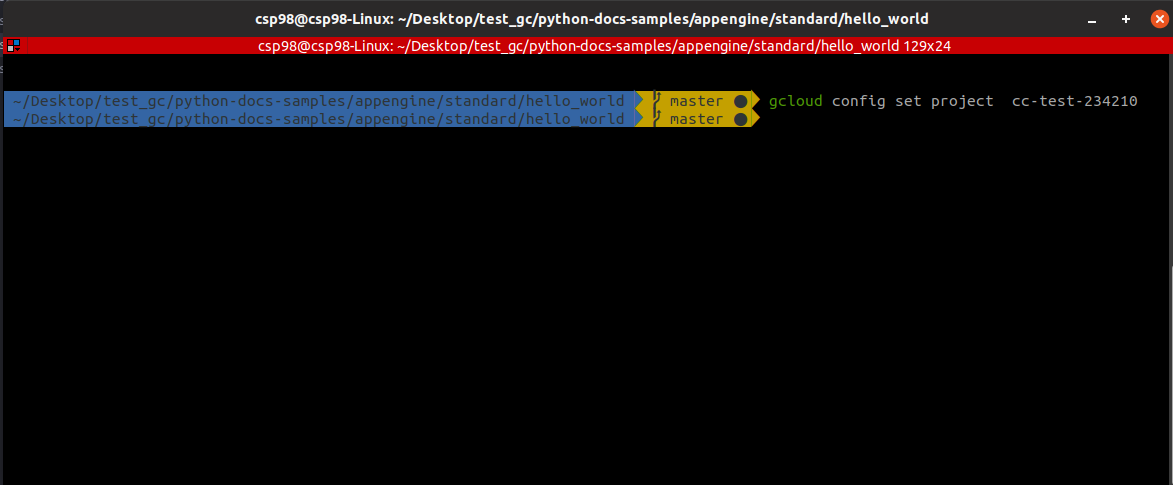
\includegraphics[scale = 0.5]{../img/tutorial/3setproject}
   \caption{Setting up the project in the SDK}
 \end{figure}

We can use the \emph{dev\_appserver.py} utility included in the GCP SDK to test the application in our local computer. This utility is modification-aware, so if we change the source code while executing it, the app will automatically re-deploy to show the changes.\\

\begin{figure}[H]
  \centering
  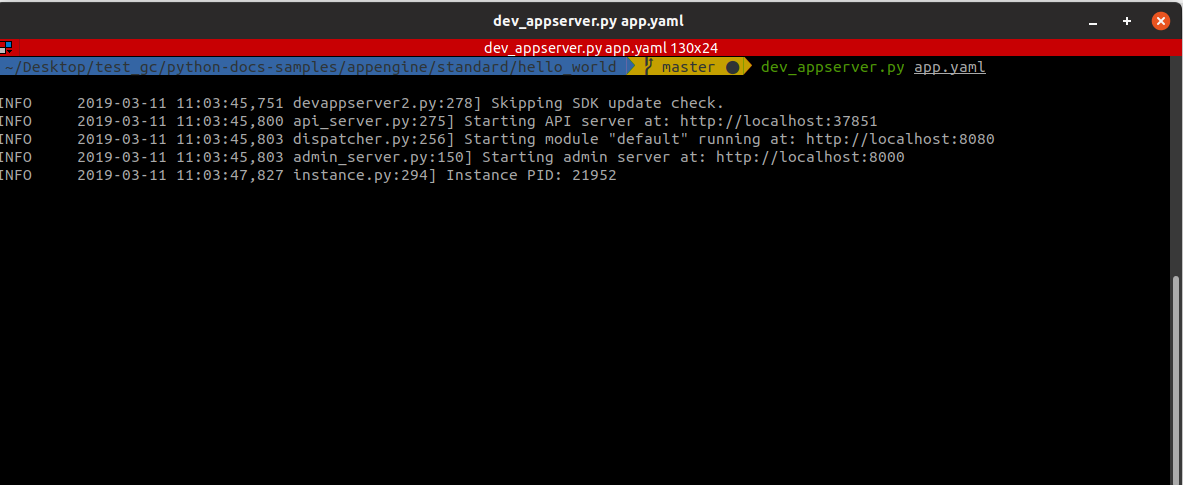
\includegraphics[scale = 0.5]{../img/tutorial/4localdeploy}
  \caption{Local deployment using \emph{dev\_appserver.py}}
\end{figure}

\begin{figure}[H]
  \centering
  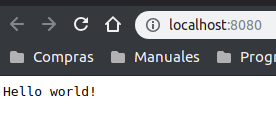
\includegraphics[scale = 1]{../img/tutorial/5localbrowse}
  \caption{Checking the local deployment}
\end{figure}

\begin{figure}[H]
  \centering
  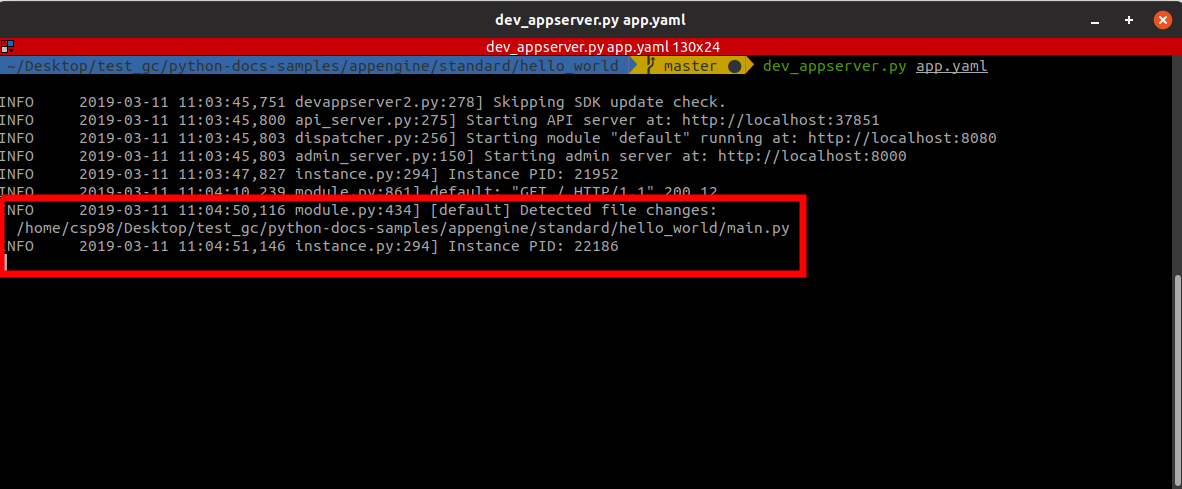
\includegraphics[scale = 0.38]{../img/tutorial/6modify}
  \caption{Detection of the modifications}
\end{figure}

\begin{figure}[H]
  \centering
  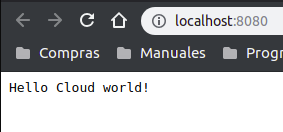
\includegraphics[scale = 1]{../img/tutorial/7browsemodify}
  \caption{Refreshing the local deployment to see the changes}
\end{figure}

When the app is finished, it's time to deploy it. We just have to type \emph{gcloud app deploy}. We will see a summary of the properties of the project. After the process finishes, the app is ready on the specified website.

\begin{figure}[H]
  \centering
  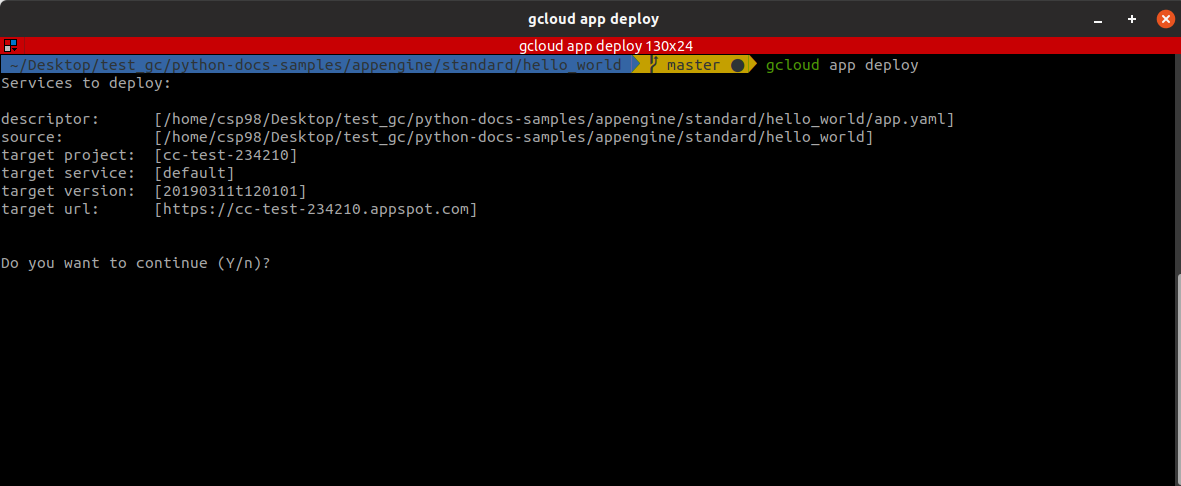
\includegraphics[scale = 0.5]{../img/tutorial/8deploy}
  \caption{Summary of the project}
\end{figure}

\begin{figure}[H]
  \centering
  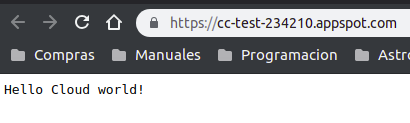
\includegraphics[scale = 1]{../img/tutorial/9browse}
  \caption{Browsing the project URL}
\end{figure}

\newpage

\begin{thebibliography}{9}

\bibitem{webpage}
Course Webpage
\\\texttt{https://www.iit.bme.hu/}

 \bibitem{tutorials}
 \texttt{https://cloud.google.com/appengine/docs/standard/python/how-to}

 \bibitem{whatis}
 \texttt{https://medium.com/@retomeier/what-is-googles-cloud-platform-d92a9c9e5e89}

 \bibitem{tuto}
 \texttt{https://cloud.google.com/appengine/docs/standard/python/quickstart}

\bibitem{companies}
\texttt{https://cloud.google.com/customers/}

\bibitem{containers}
\texttt{https://searchitoperations.techtarget.com/tip/What-are-containers-and-how-do-they-work}


\end{thebibliography}



\end{document}
